\documentclass[a4paper]{scrartcl}
\usepackage[T1]{fontenc}
\usepackage[utf8]{inputenc}
\usepackage[german]{babel}
\usepackage[hidelinks]{hyperref}
\usepackage{graphicx}
\usepackage[nomessages]{fp}
\usepackage{listings}

% TODO: Define default listing style

\usepackage{natbib}

\begin{document}
\author{Lucas Hinderberger}
\title{Beleg Programmierung I}
\subtitle{GTK-basierte Materialverwaltung}

\maketitle
\newpage

\tableofcontents
\newpage

\section{Über dieses Dokument}

Dieses Dokument stellt die begleitende Dokumentation meiner Belegarbeit im Modul Programmierung 1
im Wintersemester 2016/17 an der HTW Dresden dar.

Es soll die entscheidenden Schritte im Verlauf der Entwicklung des Beleges dokumentieren und
nachvollziehbar machen.

\subsection{Vorgehensmodell}
TODO QUELLE: Lichter Software Engineering!!!

Die Entwicklung erfolgte nach dem Wasserfall-Modell (ausgenommen der Wartungsphase, da die abgelieferte Software
nur ein akademisches Beispiel darstellt und nicht praktisch eingesetzt wird), leicht modifiziert durch den Vorzug der
Unit-Tests in / vor die Implementierungsphase (Test Driven Development). Dementsprechend ist auch dieses Dokument
in die Abschnitte ``Analyse'', ``Entwurf'', ``Implementierung'', ``Test'' und ``Inbetriebnahme''
unterteilt, um die einzelnen Stationen entlang des Entwicklungsprozesses geordnet abzubilden.

Das Wasserfall-Modell erschien -- trotz, dass es in der Praxis als veraltet angesehen wird -- als geeigneter
Entwicklungsprozess, da an der Software weder inkrementell Verbesserungen vorgenommen noch zukünftige etwaige
``Kundenwünsche'' erfüllt werden müssen. Die Aufgabenstellung (vgl. \ref{aufgabenstellung}) ist vielmehr klar und
unveränderlich, die Abnahme des Belegs erfolgt einmalig und nicht im Rahmen von ``Feedback-Schleifen'', wie sie in
der iterativen / agilen Software-Entwicklung üblich sind.

Zwar ist die Notwendigkeit des strukturierten Vorgehens nach einem Prozessmodell (selbst, wenn es ein ``Minimalmodell''
wie das Wasserfallmodell ist) und die ausführliche Dokumentation für einen Grundlagenbeleg durchaus zu hinterfragen,
jedoch erachte ich beides für sehr hilfreich und -- da in der Praxis bewährt und lieb gewonnen -- auch ein Stück weit für
unverzichtbar. Weiterhin bin ich der subjektiven Überzeugung, dass nur so ein gewisser Qualitätsstandard gehalten werden
kann, den ich aus der Praxis (überwiegend) gewohnt bin und dem ich mich auch im Studium verpflichtet fühle.
Die Erfahrungen aus der Anfertigung der Belegarbeit haben dies erneut bestätigt -- so wären beispielsweise viele, teils
hoch kritische, Fehler betrefflich der Datenintegrität nicht, oder erst spät aufgefallen, hätte ich z.B. nicht nach dem
Prinzip des Test Driven Development gearbeitet. Auch der ``Rote Faden'', den Spezifikation und Grobentwurf bieten,
hat sich während der Implementierung immer wieder als höchst hilfreich erwiesen; der hierfür nötige Mehraufwand hat sich
meines subjektiven Erachtens nach gelohnt.

\section{Analyse}
\subsection{Aufgabenstellung und direkte Anforderungen}
Zu bearbeiten war Aufgabe Nr. 2, unter Verwendung von Methode Nr. 1, errechnet aus der Matrikelnummer.
Die Aufgabenstellung des Belegs besagt in diesem Fall, dass eine Materialverwaltung unter Verwendung der GTK-Bibliothek
für die Benutzeroberfläche programmiert werden soll.

\bigskip

\noindent
Aus der online verfügbaren, vollständigen Aufgabenstellung\footnote{\url{http://www.informatik.htw-dresden.de/~beck/PSPI/Belegaufgaben/},
abgerufen am 8.12.2016} können folgende direkte Anforderungen entnommen werden:

\begin{itemize}
\item Das Programm soll Datensätze verwalten -- also anlegen, sortiert tabellarisch auflisten, suchen, bearbeiten,
löschen sowie einzelne Datensätze anzeigen -- können
\item Ein Datensatz besteht hierbei aus Artikelbezeichnung, Artikelnummer und Lagerbestand
\item Die im Programm erfassten Daten sollen im Dateisystem gespeichert (bzw. davon wieder ausgelesen) werden können.
Hierbei ist nach klärendem Gespräch auch die Benutzung des Datenbanksystems SQLite erlaubt.
\item Der Lagerbestand soll explizit über einen gesonderten Menüpunkt veränderbar sein
\item Beim Verlassen der Anwendung sollen Daten, die sich während des Programmablaufs geändert werden
gespeichert werden können.\footnote{Hierbei wird dem Anwender eine Wahl gelassen werden, ob er wirklich speichern, oder
das Programm ohne Berücksichtigung der vorgenommenen Änderungen verlassen möchte}
\item Für die Umsetzung der Benutzeroberfläche muss zwingend die Bibliothek GTK+ verwendet werden
\item Es wird ein modularer Aufbau vorausgesetzt - Das Programm ist in mehrere sinnvolle, einzeln kompilierbare Module
zu unterteilen\footnote{Dies schließt m.E.n. nicht die Nutzung gemeinsamer Typdefinitionen und Schnittstellen aus}
Hierbei sind mindestens drei Module anzufertigen
\item Quelltexte sind sorgsam zu dokumentieren -- insbesondere ist die Urheberschaft im Programmkopf zu
kennzeichnen\footnote{Bei der Quellcodedokumentation richte ich mich nach \cite[Kap.4]{Martin:CleanCode}}
\item Das Programm muss auf den Laborrechnern der Fakultät Informatik an der HTW Dresden übersetz- und ausführbar sein.
\item Teil der Aufgabenstellung ist die verpflichtende Verwendung dynamischer Speicherverwaltung per malloc/free\footnote{
Ich werde den Einsatz von malloc/free dennoch auf das Notwendigste begrenzen, da gerade unter C die dynamische
Speicherverwaltung erfahrungsgemäß eine ergiebige Fehlerquelle darstellt.}
\end{itemize}

\subsection{Ergänzende Anforderungen}
Das oben genannte Minimum möchte ich außerdem noch um folgende Anforderungen ergänzen, die sich bei näherer Betrachtung
der Aufgabenstellung als sinnvoll und einfach umzusetzen bzw. allgemein als bewährte Verfahrensweise herausgestellt haben.

\begin{itemize}
\item Die Benutzeroberfläche soll selbsterklärend und fehlertolerant sein und möglichst wenig (also ideal überhaupt keine)
Nutzerdokumentation erfordern
\item Das Programm -- insbesondere die Module für Abstraktion, Speicherung und Verwaltung von Datensätzen (vgl.
Abschnitt \ref{kernschicht} "\nameref{kernschicht}", S. \pageref{kernschicht}) -- soll möglichst umfassend durch automatische Softwaretests abgedeckt werden.
Hierbei soll nach Möglichkeit auch das Vorgehen der Testgetriebenen Entwicklung (TDD) erprobt werden.
\item Dem Nutzer soll es ermöglicht werden, optional zu einem Datensatz auch ein Bild zu speichern
\item Die in GTK+ vorhandenen Schnittstellen zur Internationalisierung sollen genutzt werden.\footnote{Selbst wenn das
Programm praktisch gesehen wohl einsprachig bleiben wird, ist dies noch immer der für GTK+-Anwendungen übliche Weg
und mit vernachlässigbar wenig Mehraufwand umsetzbar.}
\item Änderungen an den Datensätzen sollen im Arbeitsspeicher gehalten und erst mit Senden des Speicherbefehls in das
Dateisystem geschrieben werden. Wird kein Speicherbefehl gegeben (auch nicht auf Nachfrage beim Verlassen der Anwendung),
so haben diese Änderungen zu verfallen.
\item Einzelne Änderungen sollen hierbei auch wieder rückgängig gemacht werden können, solange das Programm nicht
geschlossen wurde (Strg-Z)
\item Das Speichern der Datenbankdatei soll auch unter neuem Dateinamen erfolgen können.
\item Der aktuell angezeigte Datensatz bzw. die aktuell angezeigte Auflistung sollen, wenn möglich, in ein CSV-basiertes
Format exportierbar sein.
\end{itemize}

\newpage
\subsection{Domänenmodell}
Ein einfaches, objektorientiertes Domänenmodell, welches obige Anforderungen unter Vernachlässigung dynamischer Aspekte
und Implementierungsdetails visualisiert, kann wie folgt aussehen:

\begin{center}
\noindent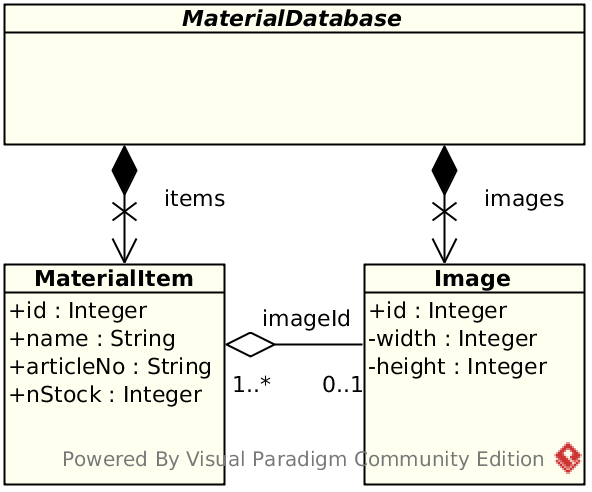
\includegraphics[width=110mm,keepaspectratio]{images/01-domaenenmodell.png}
\end{center}

Mögliche Erweiterungen dieses Modells für die Zukunft könnten beispielsweise die Katalogisierung der Materialdatensätze
in einem Kategoriebaum oder das Hinzufügen weitere Metadaten (u.A. auch Bilder) zu einem Datensatz sein.

\newpage
\subsection{Anwendungsfälle}
Die Kernanwendungsfälle, welche aus den Anforderungen entnommen werden können sind in folgendem Diagramm dargestellt:

\begin{center}
\noindent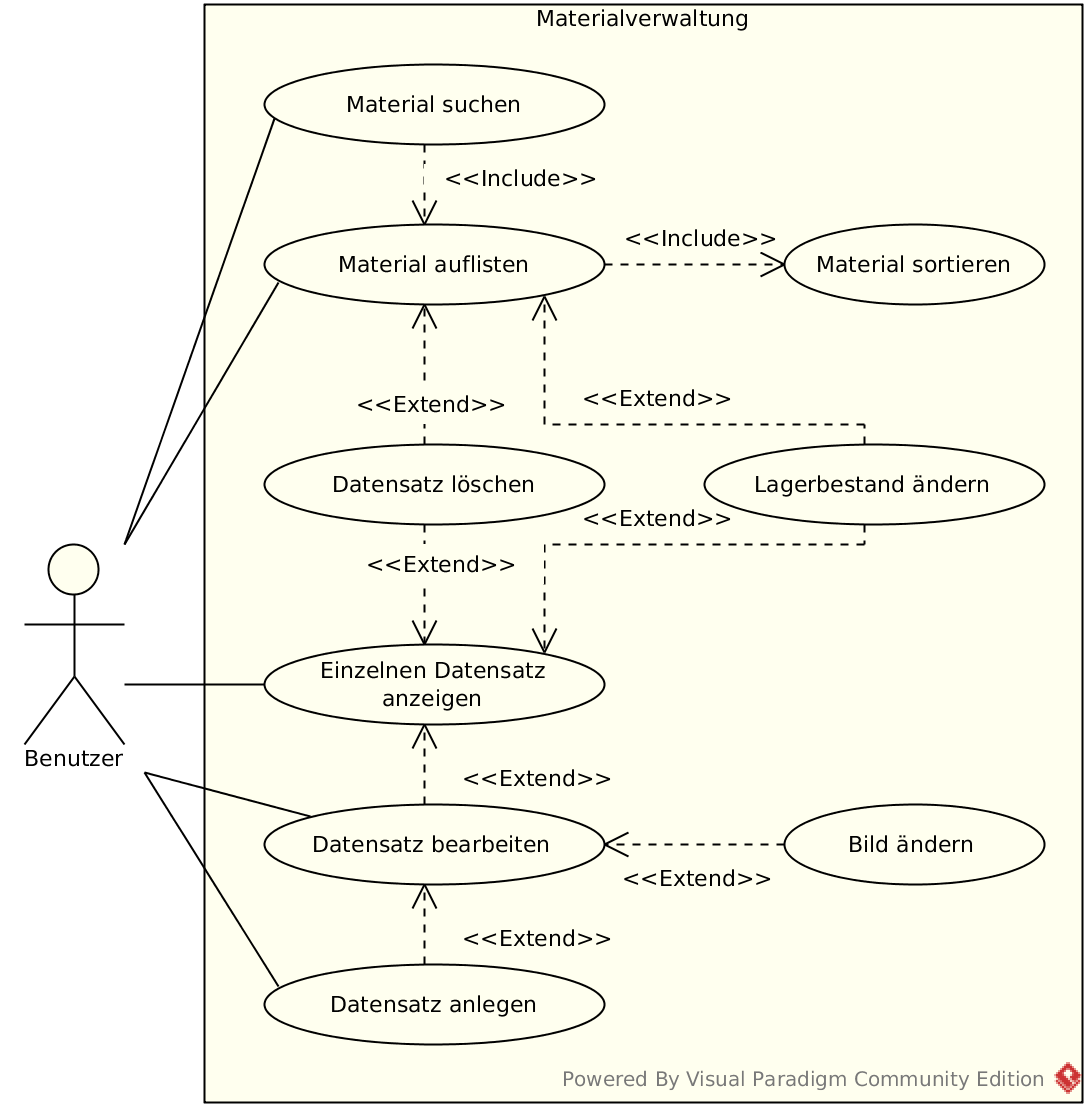
\includegraphics[width=150mm,keepaspectratio]{images/02-anwendungsfaelle.png}
\end{center}

Bereits hier zeigt sich eine möglicherweise sinnvolle Aufteilung in zwei Ansichten: Eine Such- und Katalogansicht,
sowie eine Detailansicht für einzelne Datensätze. Somit können sich beispielsweise Suche, Sortierung und Auflistung der
Materialdatensätze große Teile des Codes teilen und auch die Nutzeroberfläche bleibt in weiten Teilen kohärent und
für den Nutzer einleuchtend.

Eine Ausnahme stellt die Änderung des Lagerbestands dar: Dieser Anwendungsfall sollte von
beiden Ansichten aus erreichbar sein, denn der Lagerbestand wird im Vergleich zu allen anderen Teilen des Datensatzes
wohl mit Abstand am Häufigsten veränderbar sein und sollte daher mit möglichst wenig Aufwand auch aus der Übersichtsliste
erreichbar sein. Nichtsdestotrotz muss sich der Lagerbestand aber auch aus der Datensatz-Detailansicht heraus verändern
lassen können, soll diese doch eine vollständige Repräsentation und Manipulation eines einzelnen Datensatzes ermöglichen.

Doch auch das Löschen eines Datensatzes sollte aus beiden Ansichten heraus erreichbar sein. Zum Einen gehört es
zu einer vollständigen Datensatzmanipulation hinzu, dass ein Datensatz auch gelöscht werden kann, andererseits möchte
man als Nutzer einer Software nicht immer erst die Detailansicht eines Datensatzes aufrufen, um diesen (oder gar mehrere)
zu löschen.

Triviale Anwendungsfälle, welche keiner weiteren Erläuterung bedürfen, wurden in diesem Diagramm nicht berücksichtigt.
\section{Entwurf}
\subsection{Schichtenarchitektur}
Die Anwendung wird in drei Schichten unterteilt, in aufsteigender Reihenfolge sind
dies die Datenabstraktionsschicht, die Anwendungslogikschicht und die Darstellungsschicht. Die
hierbei erkennbare Nähe zum ``Model View Controller''-Entwurfsmuster\footnote{siehe
\url{https://de.wikipedia.org/wiki/Model_View_Controller}} ist beabsichtigt und
im Hinblick auf die (hypothetische) nächste Ausbaustufe dieser Software --
nämlich den Schritt hin zu einer verteilten Multi-User-Anwendung, z.B. durch eine
über das Netzwerk angebundene, gemeinsam genutzte Datenbank -- sogar unerlässlich.

Jede Schicht abstrahiert ihre jeweilige Kernaufgabe von der nächsthöheren Schicht.
Abhängigkeiten sind jeweils nur unidirektional zwischen einer Schicht und
den darunterliegenden Schichten bzw. externen Bibliotheken erlaubt.

Eine Schicht kann -- z.B. zu Testzwecken -- komplett ausgetauscht werden; die
Schnittstelle zwischen den Schichten wird fest durch deren jeweilige Header-Files
definiert und ist unabhängig von der konkreten Implementierung. Eine
Schichtimplementierung darf insbesondere nicht Funktionalität, die über die
Standardschnittstelle hinaus geht, höheren Schichten zur Verfügung.

\subsubsection{Datenabstraktionsschicht}
\label{datenabstraktionsschicht}
Die Datenabstraktionsschicht stellt die unterste Schicht der Anwendung dar.
Ihre Aufgabe ist die Umsetzung einer prinzipiell format- und speichermedienunabhängigen
CRUD\footnote{Create, Read/Query, Update, Delete}-Schittstelle, welche alle Datensätze
(und Operationen darauf) innerhalb einer Datenbank abbilden kann.

Hierzu gehören auch abstrakte Query-Operationen (prepared Statements), die im
einfachsten Fall schlicht an die zugrunde liegende SQL-Bibliothek weitergegeben
werden.

Operationen der Datenabstraktionsschicht schreiben / lesen direkt (bzw. unerheblich
gepuffert) in die Datenbank. Hierbei ist auf Nichtverletzung des ACID-Prinzips\footnote{Siehe
\url{https://de.wikipedia.org/wiki/ACID}} zu achten --- dies wird insbesondere durch die Benutzung
von Transaktionen und -- in der Standardimplementierung -- durch das Verwenden von SQLite als
zugrundeliegende Datenbank erreicht.

\subsubsection{Anwendungslogikschicht}
Die Anwendungslogikschicht stellt der Darstellungsschicht auf hoher Abstraktionsebene Such-, Abfrage-
und Sortierfunktionen sowie eine Transaktionsverwaltung mit Historie (für die
``Rückgängig''-Funktion) und einige Helferfunktionen, die von der Benutzeroberfläche
unabhängig sind (und bleiben sollen) zur Verfügung.

\subsubsection{Darstellungsschicht}
In der Darstellungsschicht werden schließlich Nutzereingaben entgegengenommen und
Datensätze wiedergegeben. Dies wird in diesem Fall wie gefordert über GTK+ umgesetzt,
kann aber theoretisch auch z.B. über ein via REST-API angebundenes HTML5-Frontend
realisiert werden.

Es ist möglich (und auch durchaus sinnvoll), die Anwendungslogikschicht als Bibliothek
aufzubauen und zu kompilieren, um dann verschiedenste Arten von Darstellungsschichten
nur noch gegen diese Bibliothek zu linken.

\subsection{Schnittstellenentwurf}
Da sich die objektorientierte Natur der UML nur schwer vollständig auf ein C-Programm
übertragen lässt, wird an dieser Stelle auf einen Schnittstellenentwurf und ein
UML-Klassendiagramm verzichtet. Es wird auf die entsprechenden Header-Files der
jeweiligen Module verwiesen, welche problemlos im Quellcodepaket auffindbar sind.

\subsection{Datenbankentwurf}
Die relationale Datenbank, welche als Dateiformat auserkoren wurde, ist äußerst
einfach aufgebaut:

\begin{center}
\noindent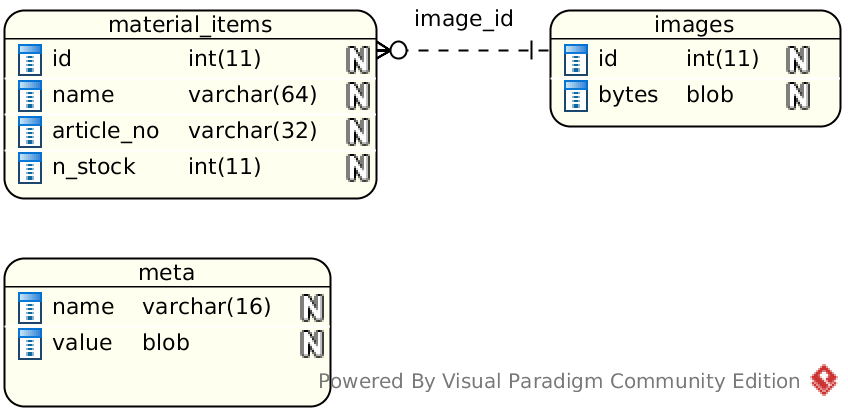
\includegraphics[width=110mm,keepaspectratio]{images/03-datenbankmodell.png}
\end{center}

Zusätzlich zum Domänenmodell ist hier lediglich die Tabelle ``meta'' neu: In ihr können
Konfigurations- und Metadaten aller Art gespeichert werden. Vorwiegend wird sie dafür
verwendet, die Version des Verwendeten Formats zu erfassen, sodass auch mit früheren
(oder späteren) Versionen der Anwendung erstellte Datenbanken verarbeitet werden können.

Der zum Aufbau dieser Datenbank erforderliche SQL-Code befindet sich bei den Quellcodes
zur Datenabstraktionsschicht.

\subsection{Anwendungsfälle und Screen Design}
\section{Implementierung}
Einige technische Fragen klärten sich erst im Verlaufe des Feinentwurfes bzw. der Implementierung.
Auf sie wird im Folgenden näher eingegangen

\subsection{Fehlerbehandlung}
Während in höheren Programmiersprachen wie Java oder C\# die Fehlerbehandlung via Exceptions standardisiert, stabil
und somit naheliegend ist, kann dies für C++ nicht uneingeschränkt\footnote{Zwar existiert für C++ eine Fehlerbehandlung
via Exceptions, allerdings ist diese für Bibliotheken nicht ohne Einschränkungen praktikabel, da Schnittstelle und
Verhalten von C++-Exceptions nicht im Standard festgeschrieben und somit vom verwendeten Compiler abhängig sind.
Da auch C++-Binärschnittstellen uneinheitlich sind, werden in der Praxis meist auch in C++ geschriebene
Bibliotheken in C-Wrapper verpackt.} und für C-Programme überhaupt nicht behauptet werden.

In der Praxis trifft man bei der Fehlerbehandlung in C-Programmen und -Bibliotheken auf verschiedenste Lösungen, vom
simplem Programmabbruch, über die Prüfung von Rückgabewerten bis hin zu Nachbauten von Exception-Mechanismen.
Während letzteres zwar großen Charme hat, ist dies für Bibliotheken -- besonders wenn diese in Binärform vorliegen
sollen -- aufgrund technischer Restriktionen (mangelnde Kompatiblität zwischen unterschiedlichen
longjmp-Implementierungen) nicht praktikabel. Gleiches gilt aus Gründen der Nutzerfreundlichkeit für den simplen
Programmabbruch.

Ich habe mich daher für die Fehlerbehandlung an der C-Standardbibliothek orientiert, welche die Rückgabe eines
Fehlerwerts, das Setzen einer \lstinline{errno}-Variablen und das Bereitstellen eines vertiefenden Error-Strings vorsieht.
Eventuellen Implementierungen von Drittparteien wird hierbei über einen privaten Header das eigene Setzen eines
dynamischen Error Strings für den \lstinline{pb_errno}-Wert \lstinline{PB_E_CUSTOM} ermöglicht.

\subsection{Abfrageschnittstelle}
TODO

\bibliographystyle{apalike}
\bibliography{dokumentation}

\end{document}